\vspace{10pt}
\subsection{JIRA Software}


\textit{JIRA Software} od spoločnosti Atlassian je software na správu projektov pre agilné tímy. Pomocou takzvaných Kanban boardov, ktoré umožňujú celému tímu vidieť aká práca ich v najbližšom období čaká, momentálne prebieha alebo je už dokončená. Jedná sa o tabuľku s kartičkami s obsahom práce, ktoré môžu následne členovia tímu premiestňovať do adekvátnych stĺpcov (obr.\ref{obr2.1}.)



\begin{figure}[ht]
    \begin{center}
        \begin{minipage}{0.99\linewidth}
            \begin{center}
                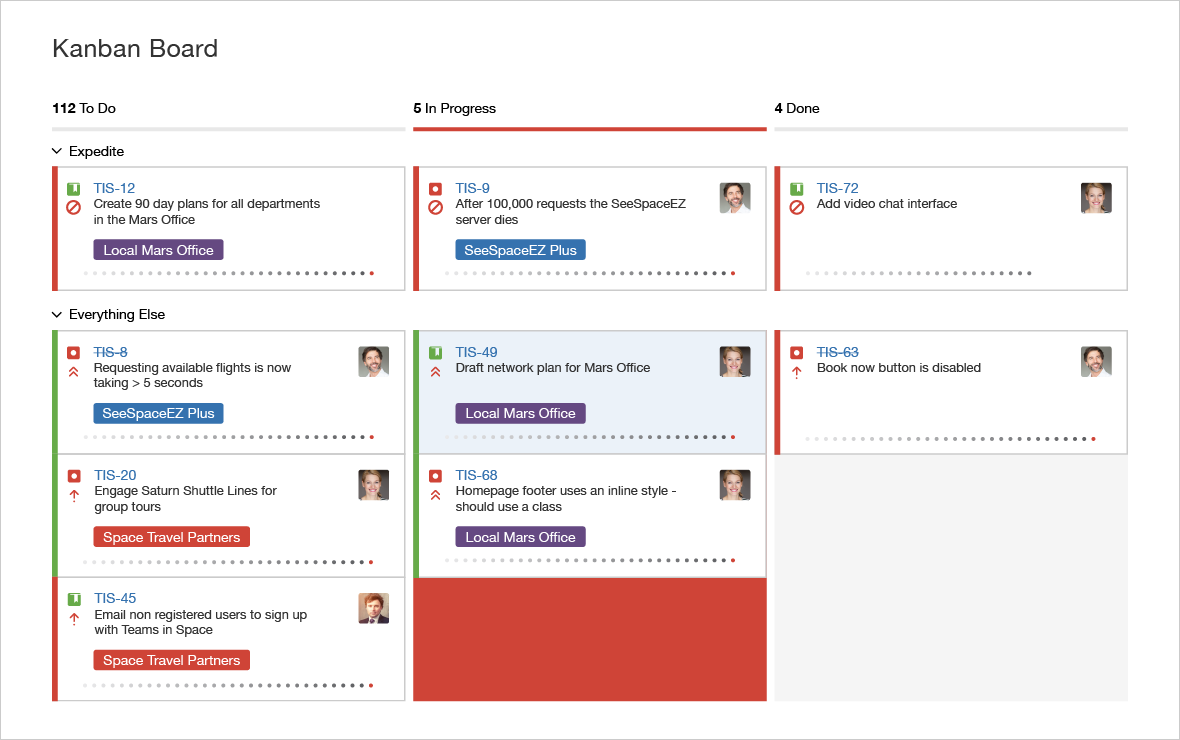
\includegraphics[width=0.99\textwidth]{images/kanbanboard.png}
                \caption{Kanban board}
                \label{obr2.1}
            \end{center}
        \end{minipage}
    \end{center}
\end{figure}

\vspace{10pt}

Každá kartička v tabuľke reprezentuje úlohu, ktorá má vždy zadávateľa a osobu, ktorá bude danú úlohu vykonávať a následne aktualizovať jej stav. Pri vytvorení a priradení úlohy príde riešiteľovi emailové oznámenie o priradení. Jedná sa o relatívne zdĺhavý proces, ktorý zamestnanci neradi vykonávajú. JIRA software je o mnoho obsiahlejší, tým pádom komplikovanejší, a napriek user-friendly prostrediu vyžaduje zaškolenie nového zamestnanca a firmy potrebujú vlastného JIRA správcu. Jedná sa ale o najobľúbenejšie riešenie pre projektový manažment ktorý umožňuje firmám lepšiu organizáciu pri riadení práce, ktorého výsledkom je kvalitný finálny produkt dodaný načas. Taktiež je rožsíriteľný o dalšie produkty spoločnosti ako sú Confluence, Bitbucket, Trello. Chýba im ale dedikovaná, jednoducha a funkčná aplikácia pre mobilné telefóny

Atlassian ponúka tri verzie ich softvéru. Verzia, ktorá sa nainštaluje na vlastný server, verzia v data centre a cloudová inštancia ich produktu. Základná verzia JIRA Core pre 25 ľudí stojí  \$1800 za serverovú aplikáciu a \$180 mesačne za cloudovú inštanciu .

\vspace{10pt}

\subsection{Slack}

\textit{Slack} je nástroj na tímovú kolaboráciu, ktorý vznikol ako interný nástroj, a v súčasnej dobe sa jedná o cloudovú službu. Jedná sa v podstate o interný chat, ktorý je rozdelený do rôznych kanálov. Kanál  (obr.\ref{obr2.2}) reprezentuje tému, projekt, lokácie alebo skupinu ľudí.


Ľudia môžu pomocou Slack-u posielať správy aj konkrétnej osobe, uskutočňovať hovory, zdieľať súbory. Externé firmy, ktoré taktiež využívajú Slack, môžu využívať spoločný kanál. Najväčšou výhodou Slack-u je, že odpadáva nutnosť odosielať hromadné maily, v ktorých sa po čase stráca prehľad, sprehľadňuje email a prenecháva mu jeho dôležitú funkciu a to  komunikáciu s  dôležitými klientmi pre formálnejší spôsob posielania správ. 
Na rozdiel od JIRA Software je Slack dostupný len z cloudu, na ktorý sa možno pripojiť cez webový prehliadač alebo aplikáciou pre všetky desktopové a mobilné platformy, pričom sa jedná o stabilné a prepracované produkty. Ponúka verziu zadarmo, ktorá ale na rozdiel od platených,  neposkytuje šifrovanie, externý prístup pre klientov alebo video konferencie.


\begin{figure}[H]
    \begin{center}
        \begin{minipage}{0.95\linewidth}
            \begin{center}
                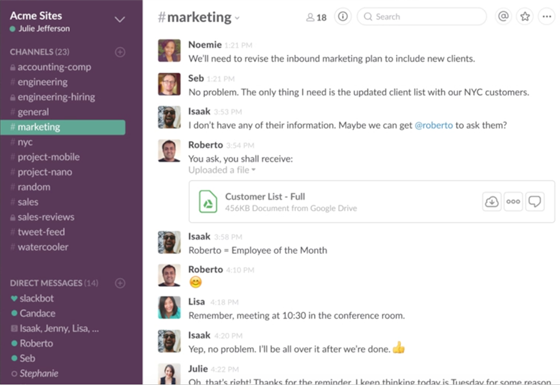
\includegraphics[width=0.99\textwidth]{images/slack.png}
                \caption{Slack, hlavné okno}
                \label{obr2.2}
            \end{center}
        \end{minipage}
    \end{center}
\end{figure}
 
\vspace{10pt}
Jedná sa o veľmi obľúbený nástroj, ktorý plní viac úlohu rýchleho chatu medzi kolegami v práci, ktorí niečo rýchlo potrebujú, ale nie sú dostatočne urgentné na telefonický rozhovor alebo posielanie mailu. 
 


\vspace{10pt}

Cieľom a úlohou tejto práce bolo navrhnúť a vytvoriť aplikáciu, ktorá by zahŕňala výhody predchádzajúcich riešení a v spojení so zadaním by bola vo finále ideálnym riešením pre malý a stredný podnik.